%\chapterimage{Figures/ArtisticView2.jpg} % Chapter heading image
%copyright: Nikhef
%authors: M.A.Bizouard, C. Palomba, C. van den Broeck, M. Maggiore
\chapter{Science Case}
\label{chap:ScienceCase}
Third-generation (3G) gravitational-wave (GW) detectors, like the Einstein Telescope (ET), will bring the {\it gravitational wave astronomy} revolution to a full realisation. Thanks to an order of magnitude better sensitivity and a wider accessible frequency band with respect to second-generation detectors, 3G detectors will allow to address a huge number of key issues related to fundamental physics, relativisitc astrophysics and cosmology. 

Astronomical sources of GWs are systems where gravity is extremely strong, and often characterized by relativistic bulk motion of massive objects. The emitted radiation carries an ucorrupted signature of the nature of the space-time geometry, and is thus an invaluable tool to understand the behaviour of matter and geometry in extreme conditions of density, temperature, magnetic field and relativistic motion.
Black holes (BHs) and neutron stars (NSs) are among the most prominent sources of GWs for Earth bound detectors. ET will uncover the whole population of coalescing stellar and intermediate mass BHs in the Universe, allowing to study subtle relativistic effects and to identify possible deviations from General Relativity in the strong gravity regime. The detection of GWs emitted by several coalescing, and possibly also isolated, NSs will finally provide the determination of NSs equation of state, and other crucial information on their properties and demography. Also, the existence of {\it exotic compact objects} will be testable.
ET will increase the chance to observe the onset of the explosion of a massive star and thus provides precious information about the explosion mecanism that gives birth to NSs or stellar-mass BHs. 
Thanks to the combined approach of multi-messenger astronomy, the NSs merger and post-merger dynamics will be unveiled and its impact on element nucleosynthesis clarified. Stochastic GW backgrounds, due to the superposition of the GWs emitted by several uncorrelated sources, are another key target of ET. The detection of a background of cosmological origin, in particular, would allow to probe very early epochs in the evolution of the Universe. 

Many of the possible achievements of ET, and other planned 3G detectors like Cosmic Explorer in U.S., are only possible through gravitational waves. For others, GW detectors are complementary to other facilities exploiting electromagnetic radiation (for instance telescopes) or other messengers, like neutrinos and cosmic rays. 

Very schematically, we can identify the following main items (divided in sub-items) as part of the ET science case.
\begin{itemize}
\item Fundamental physics
  \begin{itemize}
  \item The nature of gravity
  \item The nature of compact objects
  \item Black holes and the nature of dark matter
  \end{itemize}
\item Astrophysics of compact objects
  \begin{itemize}
  \item Neutron star properties (equation of state, demography, etc.)
  \item Black hole properties (origin, evolution, demography, etc.)
  \item Core collapse supernovae
  \item Multi-messenger astronomy (nucleosynthesis, physics of jets, cosmic rays accelerations, neutrinos)
  \end{itemize}
\item Cosmology and cosmography
  \begin{itemize}
  \item Stochastic backgrounds of cosmological origin (inflation, phase transitions, cosmic strings, etc.)
  \item Cosmological parameters (Hubble constant, dark energy density)
  \item Stochastic background of astrophysical or particle origin
  \end{itemize}
\end{itemize}
 
In the following sections we briefly discuss these scientific targets, underlying in particular what a single ET observatory could do. For much more detailed information on the 3G detectors science case the reader is referred to the 3G-GWIC Science case document.   

\section{Fundamental physics and strong field test of GR}\label{sec:fundam}

The direct detection of gravitational waves has started to give us access to the genuinely
strong-field dynamics of spacetime. This is illustrated in Fig.~\ref{fig:phasediagram}, which shows how 
different kinds of observations (past, current, and future) will give us access to different
regimes, in terms of spacetime curvature $R$ and gravitational potential $\Phi$ (which for binary 
systems can be traded for $v^2/c^2$, where $v$ is the characteristic speed of the binary and $c$
is the speed of light). 

\begin{figure}[h!]
\centering
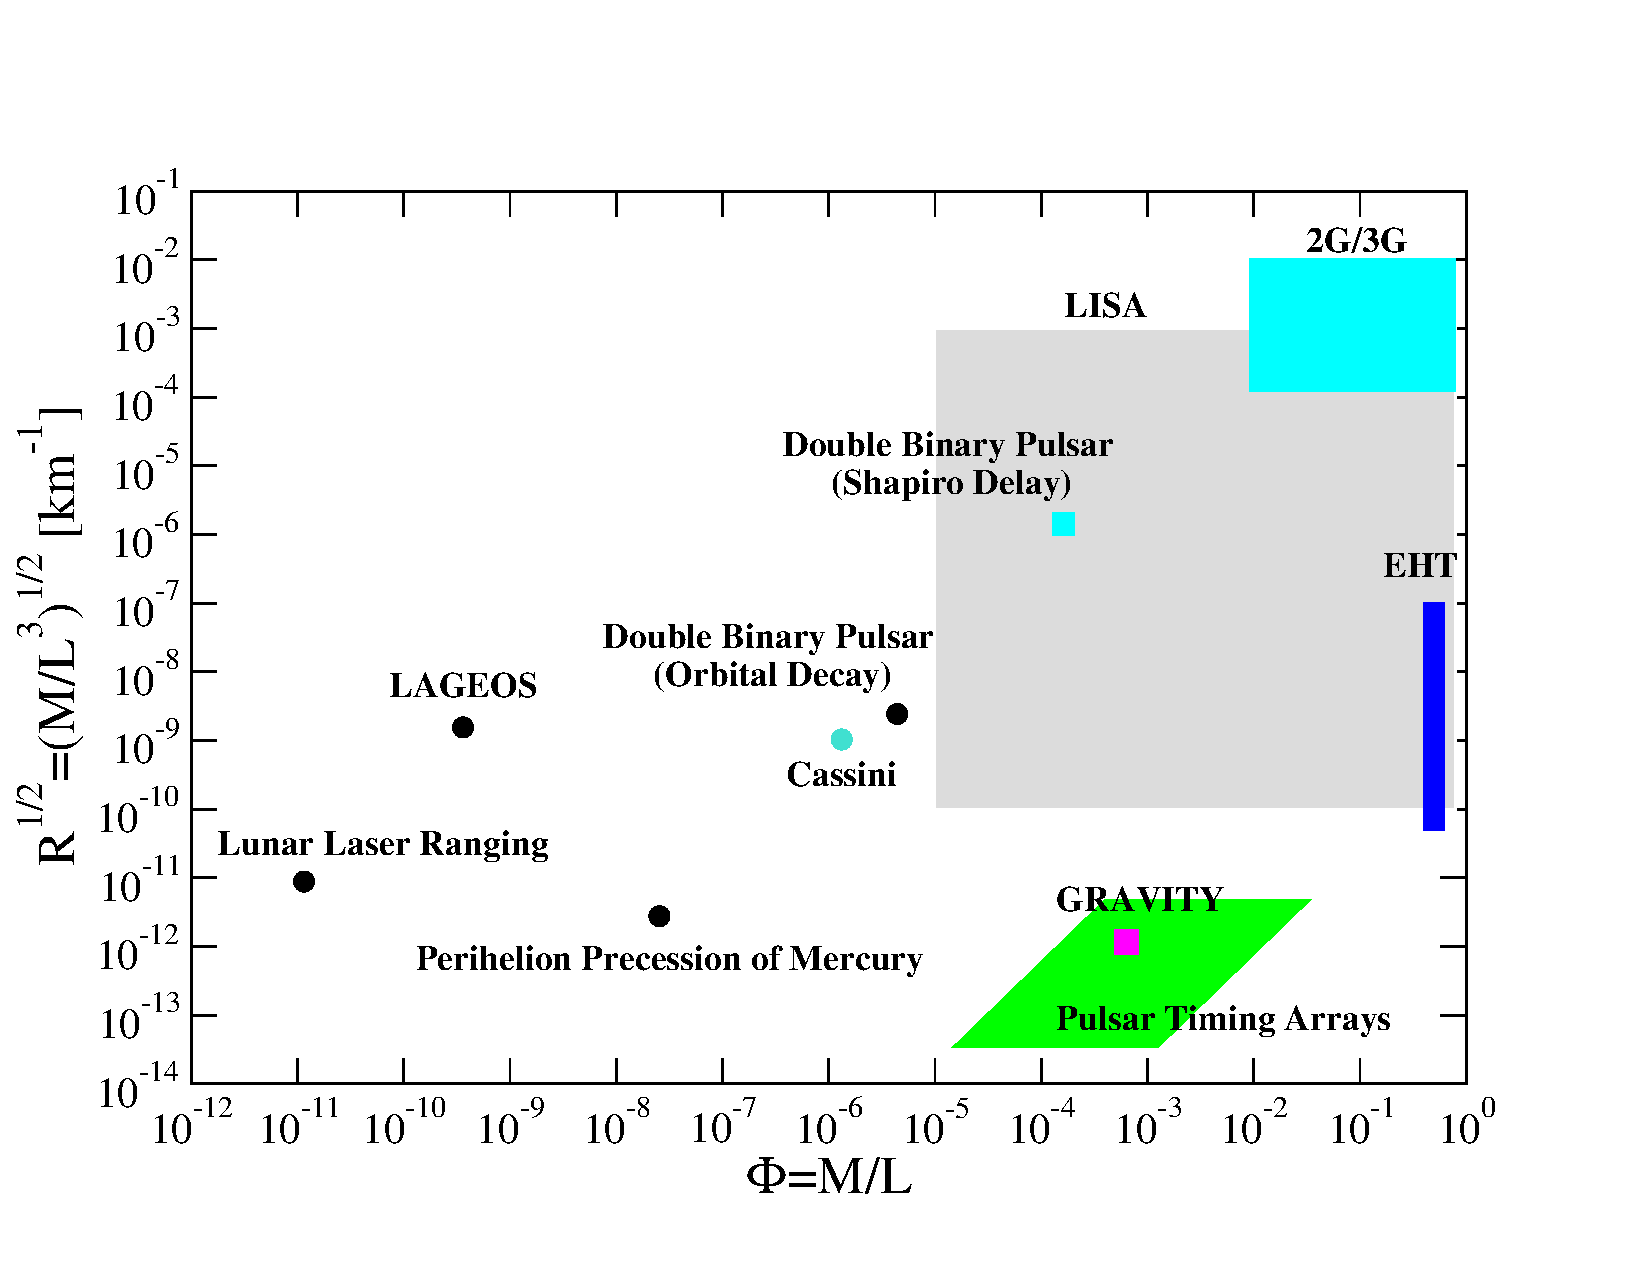
\includegraphics[width=1.0\textwidth]{Figures/phase-diagram-new4.pdf}
\caption{Probing gravity at all scales: Illustration of the reach in spacetime curvature versus potential
energy targeted through different (past, current, and future) kinds of observations. 
$M$ and $L$ are the characteristic mass and length involved in the system or process being observed. 
For binary systems binary systems, $M/L$ is related to $v^2/c^2$, where $v$ is the characteristic speed
of the binary and $c$ is the speed of light. The genuinely strong-field dynamics of spacetime 
manifests itself in the top right of the diagram.
}
\label{fig:phasediagram}
\end{figure}

Observations of gravitational waves from binary black hole and binary neutron 
star coalescences with Advanced LIGO and Advanced Virgo have enabled us to probe for the first time
the regime where both $R$ and $v/c$ are large. By observing the inspiral-merger-ringdown process
of binary black holes, we could perform a first study of the dynamics of vacuum spacetime. 
The observation of the binary neutron star inspiral GW170817 also gave us our empirical 
access to the interaction of spacetime with high-density matter. Because of the large 
distances that gravitational waves have to travel from source to observer, we were able to
strongly constrain possible dispersion that might occur; the latter led to a bound on 
the mass of the graviton of $m_g \leq 5 \times 10^{-23}\,\mbox{eV}/c^2$. This example
notwithstanding, on the whole the existing detectors lack the sensitivity to put very strong
constraints on possible deviations from Einstein's theory, particularly regarding 
the strong-field dynamics at the source, corresponding to the top right edge of 
Fig.~\ref{fig:phasediagram}. 
 
The situation will be quite different with Einstein Telescope. One reason is the much 
larger detection rate; especially for the purposes of fundamental physics, information 
from multiple sources can often be combined, and the measurement accuracy on 
common observables (e.g.~the post-Newtonian coefficients that govern binary inspiral) 
tends to improve with the square root of the number of detections. However, the fact that
the same gravitational wave source will seem much louder in ET will give us access to 
qualitatively new effects. Below we discuss in turn capabilities of ET in 
probing the properties of gravity, as well as unraveling the nature of ultra-compact
objects, with potentially game-changing implications for our understanding of black holes, 
the make-up of dark matter, dark energy, and maybe even quantum gravity itself.

\subsection{The nature of gravity}

As a result of Lovelock's theorem (Fig.~\ref{fig:lovelock}), deviations from
Einstein's theory that preserve locality must lead to additional degrees of
freedom, which generically also arise from theories of quantum gravity in the
low-energy limit. This includes higher-dimensional spacetimes, violations of the equivalence principle,  
extra fields participating in the gravitational interaction 
(\emph{e.g.}~scalar and/or vector fields in addition to the metric tensor), 
massive gravity, and violations of local Lorentz invariance; alternative theories
of gravity also often lead to extra gravitational wave polarizations in addition 
to the two polarizations of standard GR.

\begin{figure}[h!]
\centering
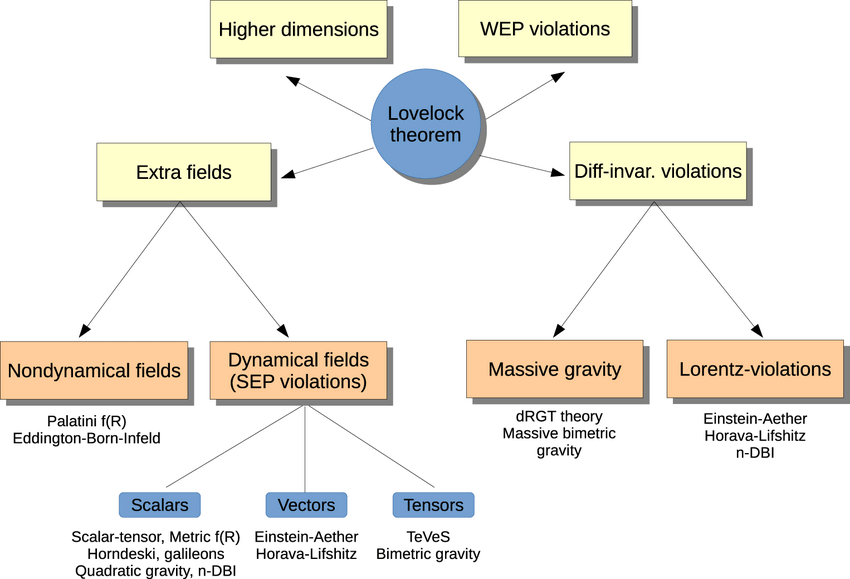
\includegraphics[width=0.9\textwidth]{Figures/Lovelock.png}
\caption{Lovelock's theorem implies that departures from general relativity 
that preserve locality must necessarily lead to new degrees of freedom 
(\emph{e.g.}~extra spacetime dimensions, extra fields, violations of the
weak equivalence principle, or violations of general coordinate invariance). 
Einstein Telescope will severely constrain -- or discover -- additional
ingredients to the understanding of gravity.
}
\label{fig:lovelock}
\end{figure} 

Theories involving additional fields often lead to violations of the strong equivalence 
principle due to their non-minimal coupling to matter. The simplest such theories are
ones with an additional scalar fields, which however could already give rise to 
exciting new phenomenology in the strong field. If the components of the binary 
acquire scalar charges, scalar waves will be emitted alongside
tensorial ones, dipolar emission would occur, and additional GW polarizations would be
present; these latter can be detected directly, or inferred from modifications of
the binary dynamics that get imprinted onto the shape of the GW signal. 

In the above we already mentioned the stringent bound on the mass of the graviton that we were able
to place with LIGO-Virgo observations; ET would improve on this by two orders of 
magnitude. Another effect that can be detected through dispersion of gravitational waves is a violation
of local Lorentz invariance. The latter is a fundamental property of the Standard Model 
of particle physics which has been tested to great accuracy in particle accelerator experiments, 
but in the gravitational sector the constraints are less refined. Since GW dispersion is
cumulative over the distance traveled, ET's ability to observe sources out to redshifts of
$z \sim 20$ will offer a much deeper probe.

Finally, we point to the possibility of parity violations in the gravitational sector, which 
occur naturally in some variants of string theory, loop quantum gravity, and inflationary 
models. This may again show up as a modification of the binary inspiral dynamics. Additionally,
parity violating theories of gravity may cause birefringence in the gravitational wave propagation; 
here too ET will profit from the ability to observe sources at extremely large distances.

\subsection{The nature of compact objects}

Various exotic compact objects have been proposed that may act as ``black hole mimickers":
boson stars consisting of bosonic fields; stars composed of dark matter particles; 
so-called gravastars whose interior de Sitter spacetime mimicks the effect of dark energy
but is held together by a shell of ordinary matter; wormholes; and, prompted by Hawking's 
information paradox, firewalls and fuzzballs for which the classical horizon is removed
through macroscopic quantum effects. When such an object is part of a binary system that undergoes
coalescence, they can make their presence known through various possible imprints on 
the gravitational wave signal that gets emitted.

During inspiral, the objects may get tidally deformed in a way that would be impossible 
for a standard, classical black hole. Unlike second generation detectors, ET will for instance be able 
to distinguish neutron stars from boson stars.  
Another possibility is that an exotic object 
has an anomalous spin-induced quadrupole moment, which would again not be accessible with 
current detectors, but measurable with ET to the percent level.

The celebrated no-hair conjecture says that a stationary, vacuum black hole is determined
by just two numbers: its mass and its spin. Stationary black holes do not emit
gravitational waves, but perturbed black holes oscillate though superpositions of
quasi-normal modes, which are damped sinusoids whose characteristic frequencies and damping times 
are again all determined by just the mass and spin of the final, quiescent black hole. If 
multiple quasi-normal modes can be distinguished, one can check for consistency between any 
three mode frequencies or damping times. Highly perturbed black holes arise as the 
remnants of binary black hole mergers. Such consistency tests will be difficult with existing gravitational 
wave detectors, but they will become possible with ET (Fig.~\ref{fig:ringdown}).

\begin{figure}[h!]
\centering
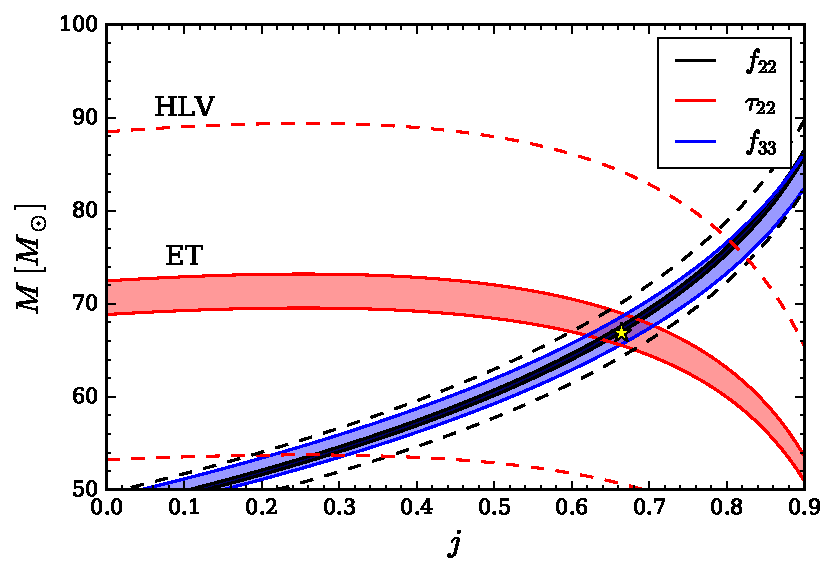
\includegraphics[width=0.9\textwidth]{Figures/3g_ringdown.pdf}
\caption{Testing the nature of black holes by using two quasi-normal modes and checking
that the characteristic frequencies $f_{22}$ and $f_{33}$ and the damping time $\tau_{22}$ are consistent
with each other, given that for ordinary black holes these can only depend on two numbers, namely
the final mass $M$ and final spin $j$. The projections are for the ``ringdown" of the remnant
black hole arising from a binary similar to the source of $GW150914$. The dashed curves 
are 95\% confidence regions one would obtain from Advanced LIGO-Virgo, while the colored bands
are for ET. The star indicates the true values of $M$ and $j$.
}
\label{fig:ringdown}
\end{figure} 

Finally, even after the ringdown has died down, exotic compact objects may continue to 
emit bursts of gravitational waves at regular time intervals, called \emph{echoes}. 
In the case of firewalls or fuzzballs, this raises the tantalizing possibility of accessing 
macroscopic quantum gravity effects. 

In short, the transition from second generation observatories to Einstein Telescope
will lead to a qualitative leap in our ability to probe both the nature of gravity
and the structure of compact objects. In addition, it may reveal the origin of dark matter, 
as we now explain.

\subsection{Black holes and the nature of dark matter}

Dark matter could be composed in part of \emph{primordial} black holes in the mass range $\sim 0.1 - 100\,M_\odot$.
These could have been produced during inflation, or from the collapse of large primordial density 
fluctuations in the very early Universe. Their mass distribution depends on the precise model 
of inflation; other processes in the early Universe such as the quantum-chromodynamic phase 
transition may also have an effect. The large number of mergers that Einstein Telescope
will see, together with its increased sensitivity, would allow us to map the black hole mass distribution
and identify an excess of black holes in certain mass intervals. For black holes with masses well below a 
solar mass, no plausible astrophysical formation mechanism is available, so that their detection would
point to the existence of primordial black holes. 
A unique advantage of Einstein Telescope
is its ability to observe stellar mass black hole mergers at redshifts of $\sim 10-20$, before
any stars had formed that could create black holes in the usual way; 
should such an event be observed then (irrespective of masses) 
the objects involved are bound to be of primordial origin.

If most of the dark matter occurs in the form of particles beyond the Standard Model, 
then also in that case gravitational wave observations can be used to find them. Black holes
could not only accrete dark matter particles, but also be subject to gravitational drag, which 
in a binary system would accumulate over the course of many orbits. If Einstein 
Telescope will be operational during the same period as LISA, joint LISA-ET observations
of the same source will then be of great value.

There is also the possibility that dark matter particles are captured in astrophysical
objects and thermalize with the star. The presence of a dark matter core in a neutron star
might again have an imprint upon the gravitational wave signal during binary inspiral and merger.
In some models, the accumulation of dark matter may lead to the formation of a black hole 
inside a neutron star, which then accretes the remaining neutron star matter, leading to 
black holes of $1 - 2 \,M_\odot$ that could be observed by Einstein Telescope.

Finally, ultralight bosons have been proposed as a dark matter candidate. If their
Compton wavelength is comparable to the horizon size of a stellar or supermassive 
rotating black hole (\emph{i.e.}~for particle masses of $10^{-21} - 10^{-11}$ eV),
they can extract rotational kinetic energy from the black hole through ``superradiance" 
to feed the formation
of a bosonic ``cloud" with mass up to $\sim 10$\% of the black hole. These clouds
annihilate over a much longer timescale than their formation, through the emission of 
nearly monochromatic gravitational waves which could be detected either directly 
or as a stochastic background from a large number of such objects throughout the Universe.
Additionally, measuring the distribution of black hole masses and spins can yield
an indication of the prevalence of superradiance through light scalars. Moreover, 
the presence of such clouds will again have an effect on binary orbital motion. 
This way gravitational waves have the potential to provide a unique probe into 
an ultralight, weakly coupled regime of particle physics that can not easily be
accessed in accelerator experiments.

\section{Astrophysics of compact objects}\label{sec:astrophy}

\subsection{Black hole binaries}
Hundreds of stellar mass BH-BH coalescences will be detected in run O3 and O4 of Advanced LIGO and Virgo detectors, with redshift up to $z\sim 1$. There are several key questions to be answered about the origin and evolution of BH-BH systems, concerning for instance, the impact of the common envelope phase in the progenitor binaries, the role of the dynamic of star clusters and galactic nuclei in producing close binaries of compact objects, the relevance of gravitational instabilities in the early Universe, which could give origin to the primordial BHs. The ET detector will observe BH-BH mergers beyond the reionization epoch, at $z \ge 6$, enabling the determination of the most relevant features, like the masses, of the first metal-poor progenitor stars and the relation between star metallicity and BH masses. As the reach of ET for BH-BH systems is well beyond the peak of the star formation density at $z\sim 2$, veryfying if the redshift dependence of the merger rate scales with the cosmic formation rate may allow to disentangle the contribution of stellar-born BHs from primordial BHs which merger rate, in contrast, is not expected to be correlated with the star formation density. Moreover, the observation of several coalescing systems could give insight on matter distribution, with BH-BH systems expected to form mainly in small and metal-poor galaxies, while primordial systems should trace the distrbution of dark matter rather than that of baryions.

The possible detection of BHs binary systems containing at least a stellar mass BH exceeding $\sim 100\,M_\odot$, or at least an intermediate mass BH (IMBH), with mass in the range $100-1000M_{\odot}$, would be of paramount importance to understand their role as {\it seeds} of supermassive BHs (SMBH), especially in conjunction with the observations by LISA. To reach this target a good sensitivity in the very low-frequency range, 1-5 Hz, will be needed.       

\subsection{Neutron stars}
NSs, isolated or in a binary system, are surely among the most important targets for ET telescope. Several aspects of these objects are still not known and can be understood thanks to the observation of GWs they emit under different circumstances. 

\subsubsection{Coalescing binary neutron stars}
The detection of GW170817 has revolutionized astrophysics and tens of more NS-NS coalescences are expected to be detected by 2nd generation LIGO and Virgo detectors in runs O3 and O4. This will help to answer crucial questions about the formation and characteristics of these systems. 3G detectors, like ET, will measure the merger rate up to redshift $z\sim 2$, where the star formation rate peaks thus allowing to probe if the redshift dependence of the merger rate is related to the cosmic star formation rate and, possibly, to place constraints on the delay time and metallicity dependence. Moreover, precise measures of the NS mass, spin magnitude and spin tilts will shed light on their origin and evolution of binary systems, more specifically providing information on the matter accretion and SN explosion. Estimating NS mass ratio {\bf \textcolor{red}{(mass or mass ratio?)}}at the $\sim 1$\% precision will be crucial to discriminate among different formation models and to get insight in the process of mass ejection which determines kilonova light curves, allowing to make comparison with models of ejection and electromagnetic emission. ET-class detectors could be also able to detect the post-merger evolution of WD-WD binarys sytems and, in particular, the merger induced collapse to NS.   

Nuclear physics theories, supported by laboratory experiments, are expected to provide a good description of matter in NS crust and in the most external part of the outer core, up to densities of about the nuclei saturation density $\rho_0 \simeq 2.5\times 10^{14}~g/cm^3$. On the other hand, the equation of state (EOS) of the outer core, up to densities of $\sim 3\rho_0$, is much uncertain and has a relevant impact on the NS radius. The star's inner core, moreover, which may undergo phase transitions involving hyperons and/or meson condensates, and de-confined quarks, heavily affects the neutron star maximum mass. While masses have been measured by radio observations for a few NSs, determination of NS radius is much more challenging due to the difficulty of modelling X-ray emission from the star's surface. 

GW170817 has demonstrated that it is possible to make very accurate measure of NS masses and, by setting constraints on the tidal deformability, has also allowed to infer a (90\% confidence interval) radius $R=11.9\pm 1.4$ km for both stars. Accuracy at the level of few percents, however, is needed in order to discriminate among between realistic EOS. Moreover, evidence for phase transitions can be achieved thanks to a sufficently detailed sampling of the mass-radius relation, which requires the detection of GWs from a population of merging NSs spanning a wider range of masses. ET can reach both goals thanks to simultaneous accurate measures of the masses and tidal polarizability of tens of coalescing NSs. 

\subsubsection{Binary neutron stars post-merger}
The merger of two NSs or of a NS-BH system is a very complex phenomenon, in which strong gravity, magneto-hydrodynamics and neutrino transport play a crucial role. Complementary GW and electromagnetic (EM) observations of GW170817, thanks to it small distance, have already provided dramatic new insight into both fundamental physics and astrophysics. GW detectors with higher sensitivity at frequencies above $\sim$1 kHz are needed, however, to directly observe the merger and post-merger dynamics. These observations will allow to shed light on the nature of the post-merger remnant, which mainly depends on the dense matter EOS, on the mass of the binary and transport properties: a BH promptly formed after the merger, a supramassive or hypermassive NS which collapses to a BH over a time scale ranging from tens of milliseconds to seconds, a long-living NS lasting for O(hours-days) or even stable. Moreover, they will allow to probe the connection between the ejecta, neutrinos and the electromagnetic signals predicted by multi-physics numerical relativity simulations. The GW observation of post-merger oscillations will provide another way to 3G detectors to measure the NS radius, with an accuracy of a few percents, comparable to that attainable in the pre-merger phase. 

\subsubsection{Continuous waves from spinning neutron stars}
A spinning NS, isolated or in a binary systyem, can also emit continuous semi-periodic GWs if asymmetric with respect to its rotational axis. Such asymmetry can derive from frozen deformations produced right affter its violent birth, from a strong enough inner magnetic field, provided it is not aligned with the rotation axis, or from non-axisymmetric motion or density perturbation due, for instance, to Ekman flow or r-modes. In case of a NS in a binary system, accretion of matter from the companion star is another viable way to produce a time-varying quadrupole moment, and then the emission of continuous GWs. The maximum degree of deformation a NS can sustain depends on the EOS: it corresponds to a fiducial ellipticity $\epsilon_{max} \sim 10^{-6}$ for standard EOS, but is expected to be much higher, $\epsilon_{max}\sim 10^{-4}-10^{-3}$, for exotic objects, containing hyperons or quark matter. In fact, it is difficult to predict the actual deformation a specific NS may own. A recent argument suggests that the typical spin-down of millisecond pulsars can be explained assuming a fiducial ellipticity of about $10^{-9}$. NS in binary systems could emit GWs as a consequence of thermally or magnetically-induced distortions, or of the excitation of r-modes. This could explain why the spin of observed NS in binary systems is significantly smaller than the theoretically maximum allowed. 

No continuous GW emission has been observed until now, and current upper limits have started to place non trivial constraints on the asymmetry level of both many known pulsars and a potential population of EM-silent NSs. ET will be sensitive to ellipticities of the order of few times per $10^{-10}$ for the nearest millisecond pulsars, and of $\sim 10^{-6}-10^{-7}$ for young pulsars. Figure \ref{fig:et_eps} shows the minimum detectable ellipticity for currently known NSs, assuming two proposed ET configurations. 
\begin{figure}[h!]
\centering
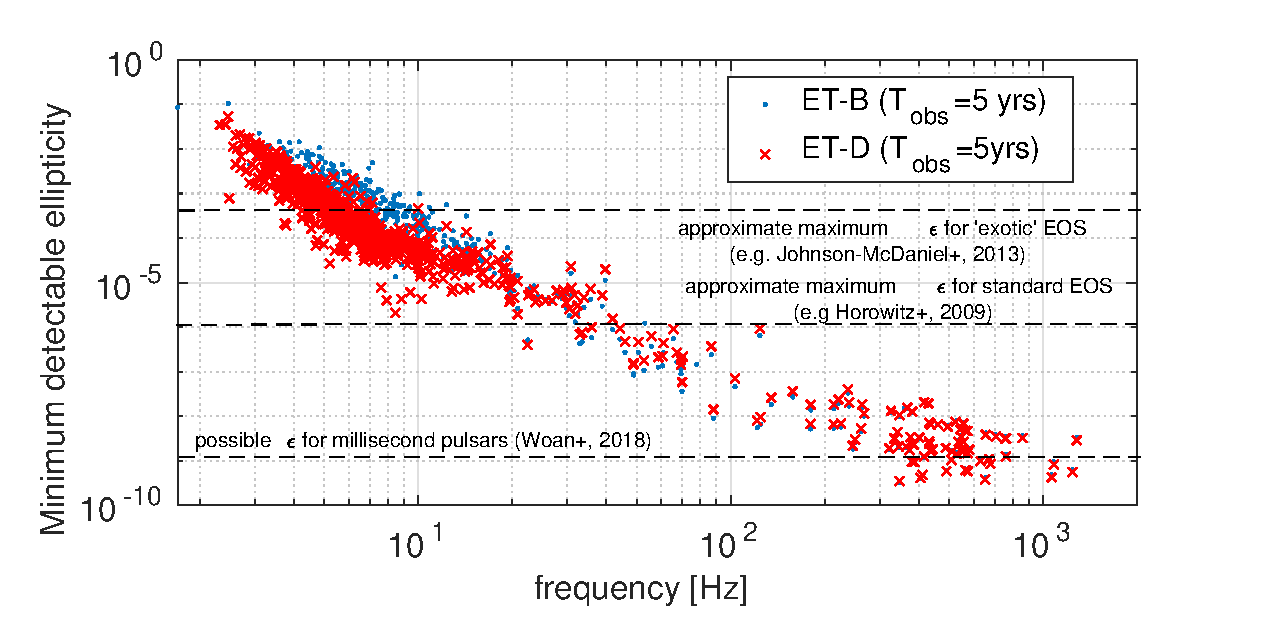
\includegraphics[width=0.9\textwidth]{Figures/ET_eps.eps}
\caption{Minimum ellipticity detectable by ET in a search of continuous waves from known pulsars, assuming an observation time $T_{obs}$=5 yrs. Two detector configurations, ET-B and ET-D, are taken into account. 
}
\label{fig:et_eps}
\end{figure} 

ET would be also able to detect CWs from at least one LMXB, Sco-X1, under the assumption that a balance among angular momentum accreted through matter infall and the emission of GWs exists. 

The detection of CW signals from spinning neutron stars will represent a complementary tool to the merger and post-merger signal for the study of the NS interior, especially if concurrent EM observations are available. It will also allow provide clues about NS formation and demography, their spin, thermal and possibly magnetic field evolution.  

\subsubsection{Burst signals from neutron stars}
Neutron stars can also emit transient bursts of GWs in association, for instance, to magnetar giant flares and pulsar glitches. Magnetars are NSs endowed with a very strong magnetic field of $10^{14}$ G or more, and are observed as anomalous X-ray pulsars AXP) or soft gamma-ray repeaters (SGR). SGRs are characterized by recurrent short-duration X-ray burst and more energetic giant flares ($10^{44}-10^{47} erg\cdot s^{-1}$ in $\sim 0.1~s$), due to global rearrangement of the inner magnetic field or of the magnetosphere. These events can induce a significant structural changes in the NS,  or excite polar oscillations, like the f-modes, causing an emission of GWs\footnote{The observation of quasi-periodic oscillations (QPO) in association to X-ray burst are commonly interpreted as torsional magneto-elastic oscillations of the NSs, which are not expected to emit GWs. They could, however, provide a strong insight in the NS structure is association with GW observations.}

Strongest pulsar glitches, like those of the Vela pulsar, are explained as due to the occasional ``unpinning'' of quantized superfluid vortices in the interior of the spinning-down NS, which move outward and release their angular momentum. The prediction on the emission of GWs are, however, still not robust due to the lack of a detailed knowledge of the process. Moderately optimistic models predict these signals can be detected by ET. 

\subsection{Core collapse supernova}
Despite the marvelous progress of the theory, the explosion mechanism is still an open question and being able to measure the dynamics of matter at the onset of the phenomena would bring invaluable information to the gravitational core collapse physics field. 
What is fairly known since the 1970's is the role of the neutrinos in the explosion mechanism. During collapse, the stellar core becomes opaque to neutrinos, producing a degenerate sea of trapped neutrinos within it, which subsequently diffuses out of the core on a timescale of order tens of seconds as the nascent proto-neutron star (PNS) cools and deleptonizes.
The three-flavor neutrino flux emanating from the PNS could power itself a core collapse supernova (CCSN) via neutrino heating on delayed timescales of order one second. This phenomena is central to most models today, with the exception of models of rare events involving significant rotation, which may be powered magneto-hydrodynamically and initiated on shorter timescales. 

GWs are generated in CCSNe by time-dependent rotational flattening, particularly during collapse and bounce, and by prompt post-shock convection, PNS pulsations, non-radial turbulent flow in the neutrino-heated bubble, the activity of the standing accretion shock instability, asymmetric emission of neutrinos and explosive mass motions, and asymmetries associated with the effects of strong magnetic fields. Relevant for the GW signature is the equation of state, the mass of the progenitor, the rate of neutronization and cooling of the core (determined in part by the neutrino opacities), and the stellar core’s initial angular momentum and mass density distributions. Measurable GW signatures of rotation require particular progenitors that rotate fast, while all other phenomena are expected to be operative in any core-collapse supernova. This broad description of the phases between bounce and explosion is now well supported by the current multidimensional numerical simulations in which all find similar features. A general consensus from all simulations is that the expected GW signal is weak (GW released energy of the order of $10^{-9}$~$M_\odot c^2$) and limits the discovery horizon of the current second-generation detectors to our galaxy. The expected galactic rate of type II/Ib supernova is also rather small (~1 per 30 years). 

The neutrino emission which will be in coincidence with the GW emission, within few milliseconds, should be detected by the current and future low energy neutrinos detectors (Super-K/Hyper-K, DUNE, JUNO, IceCube, the LVD, Borexino and KamLAND) with a higher signal to noise ratio than the GW signal and a very precise time resolution (few milliseconds) which is a fundamental information to search for a low signal to noise ratio GW signal in GW data. The false alarm rate of GW searches can be significantly improved with temporal localization given by the neutrino signal. Furthermore, there exists a strong correlation between the GW and neutrino signals as they are produced at the same interior location and will be powered by the downward accretion plumes associated with hydrodynamic instabilities present in the post-shock flow. These plumes and instabilities will modulate both signals.

The very likely diversity of the GW emission mecanisms that are at play makes the detection of a core collapse supernova GW signal very challenging. Furthermore, if the signal is likely to remain short (of the order of \unit[1]{s}), it is expected to be wide band (from few Hz up to several kHz), with very different mecanism in each frequency band. The low frequency and high frequency ET conception design is very well suited for detecting such kind of GW signal.


\subsection{Multi-messenger astrophysics}
{\bf It is not much clear to me how much having a single ET will negatively impact on multi-messenger astronomy (for transient signals).}
Prompt localization of the EM countepart of a transient (i.e. short duration) GW event is a key element for maximizing the science return of multi-messenger astrophysics. In fact, it requires a network of at least three detectors, as demonstrated by GW170817. In the case a single 3G observatory is operational at a given time, the multi-messenger science pay-off is still extremely large, although a bit reduced with respect to the case of a geographycally distributed network of detectors with similar sensitivity.
Apart from source localization, another issue to be taken into account is the discrimination among real GW signals and detector artifacts which is more difficult in the case of just one or even more detectors located in the same place. 
These problems affect, in particular, short duration transients lasting a few milliseconds - especially the unmodeled ones - while it will be less problematic for the signals associated to the coalescence of BHs or NSs binary systems, thanks to the relatively long duration of the signals in the sensitivity band of the detectors (minutes to hours). For CW emitted by spinning NSs, on the other hand, a very accurate parameter estimation - including position - can be reached with even a single detector thanks to the very specific pattern of the signals due to Doppler effect induced by the Earth motion.  
{\bf H0: can a single ET observatory allow the host galaxy EM-identification or only the statistical Hubble constant measure is viable in this case?}
{\bf Can a single ET observatory keep the pace with future powerful EM facilities?}   


     
\section{Cosmology and Cosmography}\label{sec:cosmos}


\subsection{Cosmological background}

The weakness of the gravitational interaction, that is responsible for the fact that  GW detection is such a challenging enterprise, 
also implies that the observed GW signals  carry uncorrupted information about their production mechanism. This is particularly significant for stochastic backgrounds of GWs of cosmological origin. For comparison, in the early Universe photons were kept in equilibrium with the primordial plasma by the electromagnetic interaction, and decoupled from it only at a redshift $z\simeq 1090$, when the Universe had a temperature $T\simeq 0.26$~eV. The photons that we observe today from the cosmic microwave background (CMB) therefore give a snapshot of the Universe at this decoupling epoch, while all informations about earlier epochs were obliterated by the photon collisions with the primordial plasma. Neutrinos, that interact through weak interactions, decoupled  when the Universe had a temperature $T\simeq 1$~MeV. Thus, cosmological neutrinos could carry information up to this much earlier epoch. GWs, in contrast, interact only gravitationally, and are decoupled from the primordial plasma at all temperatures below the Planck scale $\sim 10^{19}$~GeV.  Therefore a stochastic background of GWs produced in the very early Universe would give,  quite literally, a snapshot of the Universe at that epoch,
carrying informations that would be unaccessible by electromagnetic probes or by neutrinos.

Stochastic gravitational wave backgrounds, which can be of cosmological or astrophysical origin, are characterized by the normalized energy spectrum, which measures the GW energy density as a function of the frequency, by the angular spectrum, measuring the energy density at different angular scales in the sky, and by their polarization content. In order to detect a stochastic background cross-correlation among pairs of detectors is typically done. A single ET observatory, made of three non-parallel detectors, would be able to do the job.


Many cosmological production mechanisms have been studied in great detail in the literature (see \cite{Maggiore:1999vm,Caprini:2018mtu,Maggiore:2018zz} for review and references). Among the various mechanisms that have been discussed, the amplification of quantum vacuum fluctuations during inflation is particularly interesting because it would provide a direct window on inflationary physics and on the corresponding high-energy scales, and also because  it emerges from the interplay between general relativity and quantum physics. 
The stochastic background produced in   standard slow-roll inflation  is unfortunately too small even for 3G detectors. However, there are variants of the simplest models (e.g. pre-big-bang models inspired by string theory) that predict a spectrum growing with frequency, resulting in a potentially detectable signal in the ET bandwidth.
The subsequent `preheating' phase can also be characterized by violent non-linear phenomena giving rise to detectable GW production.
In the inflationary period, a detectable background could also be produced if additional fields undergo a phase of strong particle production (e.g. in the case of gauge fields coupled to a shift-symmetric inflaton). The resulting background has a single polarization and is non-Gaussian, which are very useful properties to discriminate it from other stochastic signals. 

First order phase transitions, consequence of the nucleation of true vacuum bubbles within the false vacuum filling the space as the Universe cools down, could also create a detectable stochastic background but the amplitude an characteristics of this background depends on poorly known details of the phase transition. 

Under certain conditions, so-called {\it topological defects} may be produced following a phase transition. A specific one-dimensional largely studied example of defect are {\it cosmic strings}, which are expected to form in GUTs applied to the early Universe. The GW emission is due to strings cusps and kinks following the formation of loops and basically depends, for each given model, by the string tension. 3G detectors will be able to improve 2G bounds on the string tension  by up to 8 orders of magnitudes.
      
\subsection{Astrophysical backgrounds} 
Astrophysical GW backgrounds arise from the superposition of the signals emitted by a large populations of both resolved and unresolved sources. The strongest astrophysical background, in the frequency region of terrestrial detectors, is expected to be due to the coalescence of BBHs and BNS systems, for which a normalized energy spectrum density $\Omega_{GW}\simeq 1.8 \cdot 10^{-9}$ at 25 Hz has been predicted. In fact, such background could be already detected by current 2G detectors, with ET-like detectors reaching $\Omega_{GW}\sim 10^{-12}$ in the 10-30 Hz range thus allowing, for instance, to spot anisotropies. If dark matter is partially composed of primordial black holes, with mass below $\sim 100~M_\odot$, the stochastic background they produce has an expected energy spectrum different from that of black holes of stellar origin. 
Other sources of astrophysical stochastic background are also expected, even though with a smaller amplitude, involving the galactic population of asymmetric spinning neutron stars and magnetars, or the ensemble of stellar collapse to NS or BH. One important issue is that the strong background due to merging binary systems will in fact constitute a {\it foreground} masking the smaller background of cosmological origin. As a large fraction of the merger signals will be individually detected they can be, in principle, substracted from the data thus removing the foreground. Proper data analysis techniques are being developed to this purpose, especially concerning the removal of residuals which are unavoidable due to the non perfect parameter estimation for individual signals.       

Dark matter can directly contribute to stochastic background of GWs. For instance, in U(1) extension of 
the Standard Model a spin-1 gauge boson, the {\it dark photon}, is predicted. If this particle is 
sufficiently light, it can produces an oscillating force on objects endowed with a dark charge which, 
on its turn, can bring to a stochastic GW signal potentially detectable by 3G detectors. 
Ultra-light boson clouds around spinning BH, already discussed in the context of CW signals, 
can produce a stochastic background due to the superposition of the signals produced by several 
decaying clouds.

\subsection{Cosmological parameters and dark energy}

A remarkable feature of the GWs emitted in the coalescence of compact binaries is that  they  provide an absolute measurement of the luminosity distance of the source, without the need of any `cosmic ladder' calibration. In this context coalescing binaries are called `standard sirens', the GW analogue of electromagnetic `standard candles', such as type Ia supernovae. 

The relation between the luminosity distance and redshift of the source depends on the cosmological model and is given by 
\begin{equation}\label{eq:dL(z)}
d_L(z)=\frac{1+z}{H_0}\int_0^z \frac{dz'}{\sqrt{\Omega_M(1+z')^3+\frac{\rho_{DE}(z')}{\rho_0}}},
\end{equation}
where $\rho_0$ is the closure energy density, $\rho_{DE}$ is the dark energy density and $\Omega_M$ is the current matter density. In particular, in $\Lambda$CDM, $\rho_{DE}(z)/\rho_0=\Omega_{\Lambda}$ is a constant (we neglected for simplicity the contribution of radiation, which is irrelevant at the redshifts of interest). A simultaneous measurement of the luminosity distance $d_L$ of the source and of its redshift therefore in principle allows us to extract the cosmological parameters $H_0,\Omega_M$ and to test the dark energy sector through $\rho_{DE}(z)$. GW observations, however, do not provide a direct measurement of the redshift of the source, which must be obtained either from the observation of an EM counterpart, that allows the identification  of the host galaxy - as shown with GW170817. Alternatively, with many detected signal, the $d_L-z$ relation can be tested with  statistical methods.

ET will be able to detect binary neutron star (BNS) mergers up to redshift $z\sim 2$, resulting in $10^5-10^6$ BNS events per year \cite{Sathyaprakash:2009xt}. Out of these,  in a few years of data taking one could collect $O(10^2-10^3)$ events with an electromagnetic counterpart, depending on the network of future ground-based and space-borne telescopes. For instance, performing temporal coincidences with the proposed THESEUS mission \cite{Amati:2017npy}, in 2-3 years one could detect at ET $O(100)$ GW events with an observed GRB counterpart, and several hundreds more could be detected by their soft X-ray emission~\cite{Stratta:2017bwq} {\bf please check the consistency with the multi-messenger part (MM)}. Furthermore, with such a large number of detections, the statistical method could be  quite effective even for events without observed counterpart.

In the limit $z\ll  1$, eq.~(\ref{eq:dL(z)}) reduces to the Hubble law $d_{L}(z)\simeq H^{-1}_0z$ so, from  detection of sources at low redshift,   one can measure  $H_0$.
This has been demonstrated with  GW170817, from which has been obtained the value $H_0=70.0^{+12.0}_{-8.0}\,\, {\rm km}\, {\rm s}^{-1}\, {\rm Mpc}^{-1}$~\cite{Abbott:2017xzu}.  With a large number of detections and the higher signal-to-noise ratio  of close events in ET, a much better accuracy can be reached. For instance, assuming $10^3$ standard sirens with counterpart, ET would reach an accuracy on $H_0$ better than $1\%$~\cite{Belgacem:2018lbp}.
The cosmological significance of this measurement is related to the discrepancy between the local $H_0$ measurement~\cite{Riess:2016jrr,Riess:2018uxu,Riess:2019cxk} and the value obtained from the {\em Planck} CMB data~\cite{Ade:2015xua}, that are in tension at  the $4.4\sigma$ level. While the local measurement is basically  independent of the cosmological model, the CMB observations can be translated into a measurement  of $H_0$ only after assuming a cosmological model. The $4.4\sigma$ discrepancy occurs if one  assumes a standard  $\Lambda$CDM model. Thus, this tension could be a signal of deviations from 
$\Lambda$CDM, in particular in the dark-energy sector, since a `phantom' dark energy (DE) equation of state can reduce or eliminate the discrepancy. 
The current accuracy on $H_0$ from the measurement with the single standard siren GW170817 is not accurate enough to discriminate between the local measurements and the {\em Planck}  value. However, the accuracy that can be reached with ET would allow to arbitrate the tension.

Even  more interesting is the fact that ET will have access to standard sirens at redshifts $z> 0.4-0.5$, where the effect of the DE density $\rho_{DE}(z)$  becomes visible in eq.~(\ref{eq:dL(z)}), allowing to obtain an independent  measurement of the DE equation of state, at a level comparable with that from electromagnetic observations~\cite{Sathyaprakash:2009xt,Zhao:2010sz}. In fact, recent work has shown that the situation for 3G detectors is even more interesting due to a phenomenon of modified GW propagation (see \cite{Belgacem:2017ihm,Belgacem:2018lbp} and references therein). Indeed, the natural theoretical framework for having a  dark energy sector different from a simple cosmological constant is provided by modifications of GR at the cosmological scale. In a generic modified gravity theory the cosmological evolution of the background is different from that of $\Lambda$CDM, and this is encoded in a non-trivial dark-energy density $\rho_{DE}(z)$
[or, equivalently, in the DE equation of state $w_{DE}(z)$)]. On top of this, cosmological perturbations will also be different. The modification in the scalar perturbation sector  will affect the predictions for the growth of structures or lensing, and are among the  targets of future experiments such as Euclid, DESI or SKA. The modification in the tensor perturbation sector will instead affect the propagation of GWs over cosmological distances. In GR, in the propagation across cosmological distances, the GW amplitude scales as the inverse of the scale factor, $h\propto 1/a$, which eventually results in the fact that the GW amplitude from coalescing binaries at cosmological distances is proportional to $1/d_L(z)$. In  modified gravity theories (including the models where GWs propagate at the speed of light, so to comply with the limit imposed by GW170817) this behavior is changed. As a result, the GW amplitude becomes inversely proportional to a `GW luminosity distance', different from the standard electromagnetic one. This behavior turns out to be  completely generic to all the best studied modified gravity models (scalar-tensor theories, nonlocal modifications of gravity, bigravity, etc.). For most models, the deviation from GR can be parametrized in terms of two parameters $(\Xi_0,n)$  as~\cite{,Belgacem:2018lbp}
\begin{equation}
\frac{d_L^{GW}(z)}{d_L^{EM}(z)}=\Xi_0+\frac{1-\Xi_0}{(1+z)^n},
\end{equation}
being $d_L^{EM}$ the EM luminosity distance. Measuring the modified GW propagation, through its effect on the GW luminosity distance, is a very powerful probe for the dark energy sector which cannot be accessed with EM observations. By combining this with EM measurements of $H_0$ and $\Omega_M$ will allow to constrain $\Xi_0$ below 1\% (see Fig.~\ref{fig:xi0w0}), a level already smaller than the deviation from GR foreseen by various alternative gravity theories.

\begin{figure}[t]
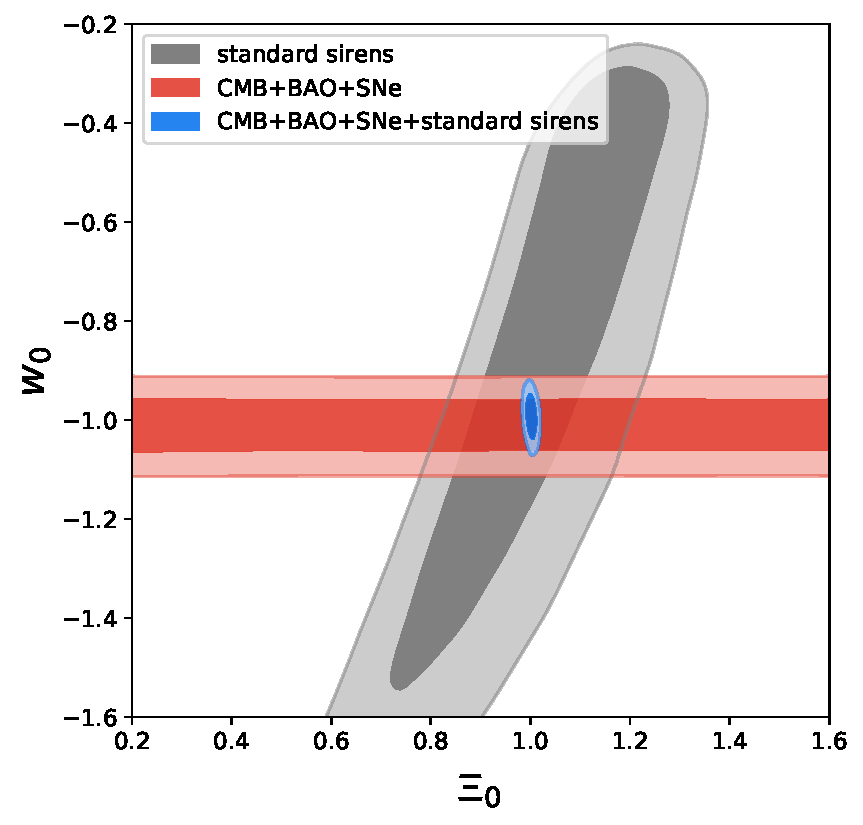
\includegraphics[width=0.45\textwidth]{Figures/xi0_w0.pdf}
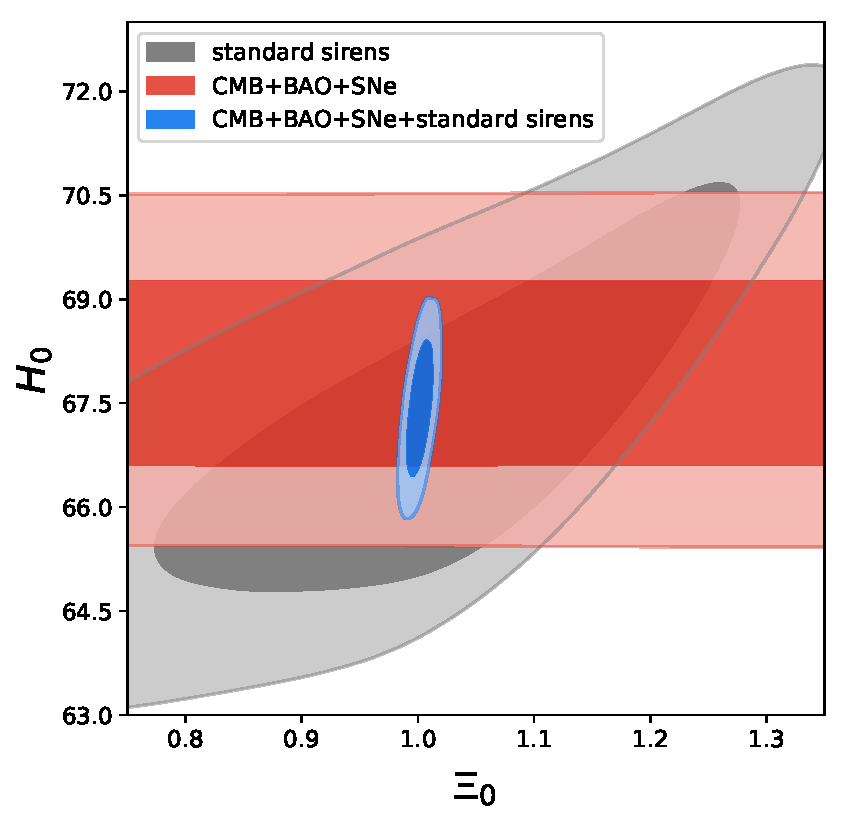
\includegraphics[width=0.45\textwidth]{Figures/xi0_H0.pdf}
\caption{The  two-dimensional likelihood in the $(\Xi_0,w_0)$ plane (left panel) and in the $(\Xi_0,H_0)$ plane (right panel), with the combined  contribution from 
CMB + BAO + SNe (red), the contribution from  $10^3$ standard sirens at ET (gray), and the total combined result (blue). (From ref.~\cite{Belgacem:2018lbp}).
\label{fig:xi0w0}}
\end{figure}

   

\section{Computing requirements}\label{compu}
The science reach of GW detectors depend on the capability to exctract from the data the biggest possible amount of information. This is strictly tied to the accuracy of the waveform models used by the analysis pipelines and to the breadth and deepness of the pipelines, which must be able to detect weak signals and estimate their parameters in a big parameter space.   
In 3G detectors, the need to detect smaller effects, which will provide information not accessible to 2G detector, and to cover a larger parameter space, to exploit their higher sensitivity and wider frequency band, makes the issue of computational requirements still crucial. 

Waveform models for 3G detectors have to include several effects currently not considered, or considered but with not enough accuracy. Among these, the presence - in binary systems - of mass components up to hundreds or thousands of solar masses, high mass ratios, up to $\sim 10^3$, arbitrary spin magnitude and orientation, tidal effects, orbit eccentricity. The richness of the corresponding waveforms will allow to distinguish among different binary formation channels and to probe their astrophysical environment. For example, including higher order harmonics in the waveform would allow - in the case of detection of an eccentric system - to break the degeneracy among distance and inclination. The study of matter at supranuclear density, which can be done analyzing NS-NS post-merger signals, needs an accurate modelling of various effects, related to the excitation of different oscillation modes, relativistic magneto-hydrodynamics, processes involving neutrinos, small-scale turbulence, etc., and the control of the associated systematics. This is an extremely difficult task which calls for big improvements in understanding the physics of NSs, in numerical relativity code development and optimization, and in computing frameworks and infrastructures. A good accuracy in the NS EOS, from the large number of expected detections, would allow, among several other things, to break the mass-redshift degeneracy opening the possibility to make cosmology without the need to identify EM counterparts of NS-NS systems. Properly modelling the tidal disruption in NS-BH systems is another relevant item which requires advancements, especially in the case of BH spin precession. Properly modeling exotic objects (ECOs), formed after a coalescence, is also crucial in order to extract as much as possible information.

For 3G detectors new challenges arise also concerning the analysis of the data. For BNS systems the signals in the detector band, which extends to few Hertz, can be $\sim$ 1 day long. This poses several non trivial problems. First, the construction of template banks for such long waveforms becomes computationally expensive. Second, the extension of the parameter space (large mass ratio, not aligned spins, eccentricity,...) largely increases the number of needed templates, and this will be a major challenge from the computational point of view. Third, the motion of the detector implies a time-varying detector response to the source location and a frequency modulation due to the Doppler effect. Both issues complicate the analysis and increase its computational cost. Fourth, with an increased distance reach, and longer waveforms, detectable signals will overlap and this must be properly taken into account.

For CW searches the computing problem will be not different in the 3G detector era respect to the current situation. All-sky searches are currently computationally bound and this forces to use hierarchical semi-coherent procedures which strongly reduce the computational cost at the price of a sensitivity loss in comparison to the optimal procedure bases on matched filtering. One major target for exploting at the best ET data will be to develop analysis algorithms able to reduce as much as possible the sensitivity loss compared to the optimal matched filter method. The sensitivity of the search for directed long-transients signals, like those emitted by long-lived NS formed after the coalescence of a BNS system, is also currently limited by the dimension of the parameter space, consequence of the fast evolution of the signal frequency. New methodologies able to improve the sensitivity are needed to overcome this problem and make the detection of such kind of signals more likely.    

  


